

% \yi{consider re-organize this section: detail on our meeting ...}

% \subsection{Research outline}
    %\subsubsection{Data preparation}
In this section, we present the work stream involved in MPC of microgrid energy management. The application of MPC consists of two main stages in this study: forecasting and optimization. In order to be coherent, we first introduce the optimization task and related concepts in Sec. \ref{section:MEM}, then detail the load forecasting in Sec. \ref{section:Building load forecasts}. 
In the initial stage, predictions for the loads are made based on historical data and other relevant information. Machine learning approaches and heuristic methods are used for forecasting in this study. Several lump metrics are included to evaluate the forecasting accuracy.
Then an optimization problem is formulated for MPC, which takes various control variables into account and is subjected to specific constraints. Its objective is to find the control actions that minimize the performance criterion (i.e., utility cost in this study). In order compare the control performance of MPC with different forecasts, we consider rule base control (RBC) as a benchmark. RBC is a controlling technique that does not rely on forecasts, based on which the concept value of information is proposed as a metric. 
At the end, two experimenting scenarios considering different billing schemes and corresponding configurations are introduced in Sec. \ref{section:configurations}.

%============================================================================================================
\subsection{Microgrid energy management} %-------------------------------------------------------------------
\label{section:MEM}
\subsubsection{System Configuration}

In this paper, we denote the set of real numbers by $\R$ and the set of integers by $\Z$. We use functions $\ind{\cdot}$, $[\cdot]^{+}$, $[\cdot]^{-}$, $\lfloor \cdot \rfloor$ in their conventional meanings, i.e., $\ind{x}=1$ if $x$ is true otherwise $\ind{x}=0$, $[x]^{+} \coloneqq \max\{0,x\}$, $[x]^{-} \coloneqq \min\{0,x\}$.\footnote{
For consistency, we adopt the convention that using lowercase letters (e.g., $x$) for (decision) variables, uppercase letters (e.g., $X$) and Greek letters (e.g., $\alpha$) for parameters, and calligraphic uppercase letters (e.g., $\mathcal{X}$) for sets.}
    
We consider a typical external-grid-connected microgrid, which is distributed with solar panel (PV) generation and battery energy storage system (BESS). The loads of the microgrid is building energy consumption. Specifically:

\begin{itemize}
    \item At time $t$, building load $\pbld_t$ and PV generation $\ppv_t$ are assumed to be uncontrollable.
    \item The microgrid can import electricity power from, or export to the external grid, which is $\pgrid_t$ at time $t$ (negative for export), at time-of-use (TOU) tariff $\tou^+_t$ (purchase) or $\tou^-_t$ (sell).
    \item A battery with capacity $B$ and maximum discharging (charging) power $\pbattU$ ($\pbattL$). At time $t$, its discharging power is $\pbatt_t$, for which negative value indicates charging.
    \item A \emph{demand charge} term is included as part of the utility bill, which has a constant marginal rate $\dc$ (per kW) applied to the maximum consumed power $\pDC$ within the billing cycle.% And the latest maximum consumed power at time $t$ is $\pDCt$.
\end{itemize}

\subsubsection{Optimal Energy Management} %------------------------------------------------------------------

\begin{subequations}
The goal of the optimization is to minimize the electricity bills over horizon $\tset = \{0,1,...,T\}$, i.e.,:
\begin{equation}\label{eq:opt_obj}
    \sum_{t=0}^{T-1} \left\{ 
           \tou_t^+ \relu{\pgrid_t} - \tou_t^- \reluN{\pgrid_t} \right\} \dt
           + \dc \, \pDC
\end{equation}
which is the consumption-based cost plus the demand charge. $\pDC = \max_t~ \{\pgrid_t\}$, which is the maximum grid import power within a billing cycle.\footnote{For simplicity, we consider $\tset$ contains one billing cycle, which is typically one month.} We can reformulate the maximum equality as:
\begin{equation}\label{eq:constr_dc}
    \pDC \ge \pgrid_t, ~~~~ \forall ~t
\end{equation}

Supply-demand balance should be observed at every time step:
\begin{equation}
    \pgrid_t + \pbatt_t + \ppv_t = \pbld_t ,
                ~~~~ \forall ~ t
\end{equation}

Power imported from or exported to external grid is limited:
\begin{equation}
   \pgridL \le \pgrid_t \le \pgridU, ~~~~\forall ~t
\end{equation}
If $\pgridL = \pgridU = 0$, the microgrid is isolated. In general, such limits are determined by the transformer capacity, per certain microgrid codes.

For the battery, the following constraints (dynamics) need to be satisfied\footnote{We consider an ideal battery model here for simplicity. We will plug in more complicated models, e.g., considering battery degradation, in our future work for sensitivity analysis.}:
\begin{align}
   & \ebatt_{t+1} = \ebatt_t  + \left(\effbatt^- \reluN{\pbatt_t} - \frac{1}{\effbatt^+} \relu{\pbatt_t}\right) \dt,
                ~ \forall ~ t \\
   & \pbattL \le \pbatt_t \le \pbattU,~~~~ \forall ~ t\\
   &  \ebattL \le \ebatt_t \le \ebattU,~~~~ \forall ~ t\\ 
   & b_0 = B_0 , ~~ b_T \ge B_T \label{eq:constr_e_init_targ}
\end{align}
where $\effbatt^+$ ($\effbatt^-$) is the discharging (charging) efficiency.

\end{subequations}

To conclude, a general formulation of optimal energy management is:
\begin{subequations}\label{eq:opt1}
    \begin{align}
        \min~~ & \text{obj. \eqref{eq:opt_obj}}\\
        \text{s.t.~~~~} & \text{constr. \eqref{eq:constr_dc}-\eqref{eq:constr_e_init_targ}}
    \end{align}
\end{subequations}
With some trivial reformulations, the program \eqref{eq:opt1} is a linear programming (LP).\footnote{Some assumptions, e.g., $\tou^+_t \ge \tou^-_t$ are required, which are also trivial.}

\subsubsection{Model predictive control (MPC)} %------------------------------------------------------------------

Compactly, we write the constrained finite-time optimal control (CFTOC) problem as:
\begin{equation}
    \widetilde{u}_{t_{[K]}} = \arg\min J(u_{t_{[K]}} \mid x_t, w_{t_{[K]}}, \theta_{t_{[K]}})
\end{equation}
where $z_{t_{[K]}} = \{z_t, z_{t+1}, ..., z_{t+K}\}$, and $x, u, w, \theta$, by convention of control literature, are states, actions, disturbances, and parameters respectively. Disturbances $w$ are unknown at the moment of solving CFTOC, so we substitute with the forecasts $\hat{w}$ in the problem formulation. Under MPC, CFTOC is solved, but we only implement the first $K^\text{exe} \le K$ steps of its solutions before re-optimize. The procedure is shown in Alg.\,\ref{alg:mpc}.  
\begin{algorithm}
\caption{model predictive control}\label{alg:mpc}
\begin{algorithmic}
\STATE $t \gets T_0$, $x_t \gets X_0$
\WHILE{$t \le T_\text{end}$}
\STATE \textbf{forecast}~$\widehat{w}_{t_{[K]}}$
\STATE \textbf{solve} $\widetilde{u}_{t_{[K]}} = \arg\min J(u_{t_{[K]}} \mid x_t, \widehat{w}_{t_{[K]}}, \theta_{t_{[K]}})$
\FOR{$k=0,...,K^\text{exe}-1$}
    \STATE \textbf{execute}~$\widetilde{u}_{t+k}$, \textbf{update}~$x_{t+k}$
\ENDFOR
\STATE $t \gets t + K^\text{exe}$
\ENDWHILE
\end{algorithmic}
\end{algorithm}

In our specific context, states $x$ are battery charge $\ebatt_t$ and the maximum imported power in the billing cycle up to $t$, denoted as $\prevmax_t$. Actions $u$ include schedules for battery charging $\pbatt_{t_{[K]}}$ and grid power exchange $\pgrid_{\tToK}$. Disturbances $w$ refer to uncontrollable PV generations and building loads, whose estimates are denoted as $\pvest_{\tToK \mid t}$ and $\bldest_{\tToK \mid t}$.

In real execution, the battery will follow what are solved from the CFTOC.\footnote{We assume that such operations are always feasible and can be precisely implemented, since we focus on the uncertainty of building load.} When building load and PV generation are realized, the microgrid imports/exports the amount of energy from the grid that synchronously balances the supply and demand (instead of executing the one solved in CFTOC with predicted load and generation). Formally:

\begin{equation}
%\begin{align}
    \pgridSch_t  = \bldest_t - \pvest_t - \pbattSch_t 
    %\label{eq:pgrid_sch}\\
    %\pgrid_t & = \pbld_t - \ppv_t - \pbattSch_t
    %\label{eq:pgrid_real}\\
    %& = \bldest_t - \pvest_t + \epsilon_t - \pbattSch_t \notag
    % = \pgridSch_t + \epsilon_t
%\end{align}
\end{equation}
% where $\epsilon_t$ is the prediction error on net load at time $t$.

\subsubsection{Rule-based control (RBC)} %--------------------------------------------------------------------------
\label{sec:RBC}
Rule-based control (RBC) is a classical and widely used control paradigm. Different from optimization-based control (e.g. model predictive control), RBC relies on predefined rules to make decisions for controlling, and does not integrate the forecasts into decision making. 
One particularly notable RBC strategy, known as 'Maximize Self-Consumption' (MSC), has found widespread application in the realm of microgrid management, particularly in systems featuring renewable energy sources. The core tenet of MSC revolves around elevating the priority of locally generated power, specifically from PV generations and BESS, with the ultimate aim of curtailing dependence on the external grid.
To be specific, PV generations will first satisfy the building load. When there is surplus power from PV, it will charge the battery, and lastly export to the external grid. When PV generations can not satisfy the energy requirement of building, the battery will discharged to provide the needed energy, and then importing from the external grid will be the last option if the power is still not enough. 
The control performance of RBC served as part of the benchmark when evaluating the performance of MPC with different forecasts.

\subsubsection{Model predictive control performance} %-------------------------------------------------------

\emph{Value of information} (VoI) is a useful concept for evaluating the impact of forecast accuracy on control performance. Let $u^*(\hat{w})$ be the control sequence implemented under MPC when the estimates for disturbances $w$ are $\hat{w}$, and $J(u^*(\hat{w}); w)$ be the realized outcome of this control sequence. We define the value of forecast $\hat{w}$ as the difference of it control performance and that when ground truth information $w$ is available, i.e.,
\begin{equation}
    V(\hat{w}; w) =  J(u^*(w); w) - J(u^*(\hat{w}); w)
\end{equation}
From the definition, $V(\hat{w}; w) \le 0$, and the higher value $V$ is, the more valuable $\hat{w}$ is for the control task. In order to make meaningful comparisons across different scenarios, we define a \emph{normalized value of information} (VoI*) as:
\begin{equation}
    \text{VoI*} = \frac{J(u^*(\hat{w}); w) - J(u^{\text{RBC}}; w)}{J(u^*(w); w) - J(u^{\text{RBC}}; w)}
\end{equation}
where $u^{\text{RBC}}$ is the control sequence made maximize self-consumption strategy as introduced in Sec. \ref{sec:RBC}. The forecast $\hat{w}$ achieves $100\%$ VoI* if it has the same control performance as MPC with ground truth forecasts (MPC-GT) and it cannot do better. Forcast $\hat{w}$ is useless if MPC with it cannot outperform a RBC strategy that does not require any forecast, in which case its VoI* is $0\%$. VoI* may even be negative, which means $\hat{w}$ provides misleading information which leads MPC to make far suboptimal actions so that it is outperformed by RBC.
%\footnote{The RBC strategy may or may not rely on forecast $\hat{w}$. For our specific choice, maximize self-consumption (MSC) strategy, it does not use forecast information.} 
%============================================================================================================



%============================================================================================================
\subsection[Building load forecasts]{Building load forecasts\footnote{For simplicity and consistency, we only consider building load forecast in this work, meanwhile assuming PV generations demand known. The error in PV generation forecasts can be easily combined with that of building load (in other words, forecasting the \emph{net} load).} }
\label{section:Building load forecasts}

%\yi{Please explicitly give ONE reference for each algorithm, where the readers are expected to find anything we omit here to reproduce the results.}

To diversify the forecasting algorithms and their forecast residual distributions, we selected two distinct categories of forecasting methods: \textit{machine learning approaches} and \textit{heuristic methods}.
Four distinct and illustrative techniques for time series forecasting were utilized in the construction of the load prediction model: linear regression (LR), extreme gradient boosting (XGBoost), probabilistic forecasting incorporating autoregressive recurrent networks (DeepAR), and the temporal fusion transformer (TFT). Model training of LR, DeepAR and TFT is carried out based on the open source software \emph{Darts} from \emph{Unit8}\cite{Darts}, and the model working for XGBoost is performed on open source software from \cite{XGBoost}. In addition, we denote MPC with machine learning forecasts by \textbf{MPC-ML}.

\subsubsection{Load data} %----------------------------------------------------------------------------------

We utilized an open source dataset obtained from the microgrid at the University of California, San Diego (UCSD)\cite{silwal_open-source_2021}. The dataset consists of building load and PV generation data spanning from 2017 to 2019, sampled every 15 minutes. After conducting the required data quality control, we selected 8 buildings that were representative, and calculated their average load as a virtual profile. The average load, denoted by $\avepbld$, was 73.6 kW. Evaluations on control performances were carried out on the data from the year 2019, while forecast models were trained (and validated) using data from 2017 and 2018.

\subsubsection{Covariates} %---------------------------------------------------------------------------------

\begin{figure}[!ht]
\centering
  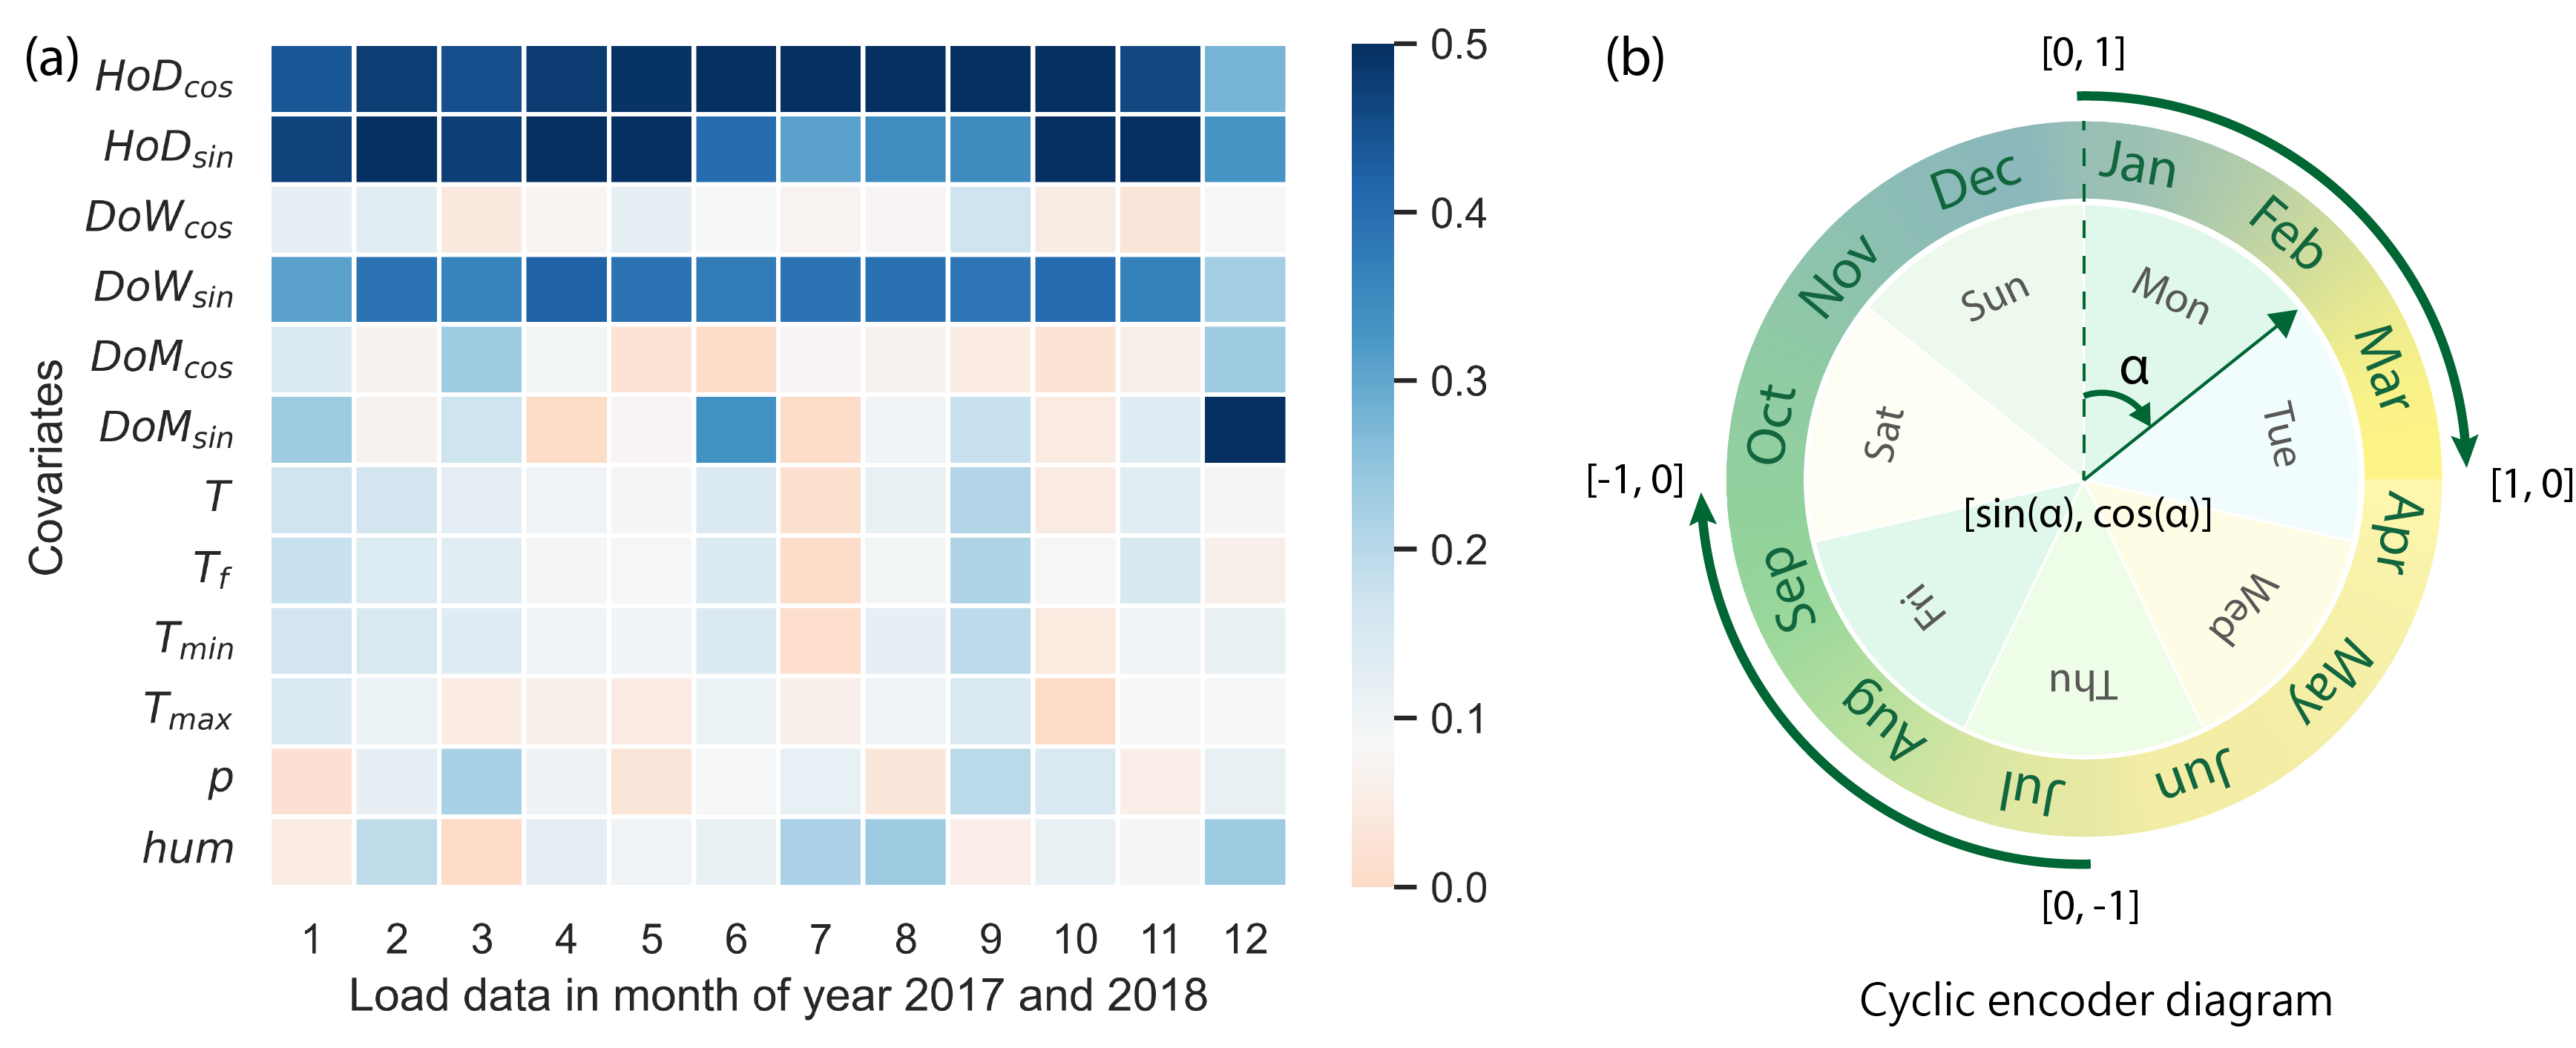
\includegraphics[width=0.85\textwidth]{figures/Pearson_correlation_and_cyclic.png}
  \caption{\textit{Pearson correlation and cyclic encoder diagram} \textbf{(a)}. Absolute Pearson correlation values between covariates and load data in a month. Month is given in $x$-axis and type of covariates labeled in $y$-axis. Deeper blue indicates higher value of correlation, and orange indicates value below 0.1. \textbf{(b)}. The diagram shows the encoding rule of cyclic encoding. For simplicity, only month of year (MoY) and day of week (DoW) are shown in the diagram. }
  \label{fig:pearson_cyclic}
\end{figure}


In the context of the forecasting tasks of this study, covariates pertain to external data that can be utilized as inputs for model enhancement seeking to improve forecasts. These external data encompass meteorological data ($\mathbf{CO^M}$) and time feature data ($\mathbf{CO^T}$).  The target to predict is the series of building loads, and the covariates themselves are not predicted. 

%\footnote{More information about meteorological data we used is provided in the Appendix. }
\emph{Meteorological data} was retrieved from \emph{OpenWeather} with an hourly granularity. The measured data includes: ambient air temperature ($\mathbf{T}$, ℃), feels-like temperature ($\mathbf{T_f}$, ℃), atmospheric pressure ($\mathbf{p}$, mmHg) and relative humidity ($\mathbf{hum}$, \%). Having perceived that the daily load patterns of the profile are associated with the activity intensity during workday or holiday, we encode \emph{time feature} covariates including hour of day ($\mathbf{HoD}$), day of week ($\mathbf{DoW}$), month of year ($\mathbf{MoY}$) and day of month ($\mathbf{DoM}$). These inputs use a cyclic encoder (see Fig. \ref{fig:pearson_cyclic}-\textbf{b}), which can help the model describe the periodic temporal features more objectively compared with the integer and one-hot approaches\cite{cyclic_encode}. Furthermore, a boolean variable ($\mathbf{D_{work}}$) is included to indicate whether the day is a workday.

As shown in Fig. \ref{fig:pearson_cyclic}-\textbf{a}, most covariates we selected have correlation value higher than 0.1. Among all covariates, time features, particularly $\mathbf{HoD}$ and $\mathbf{DoW}$, show strong relations with monthly load data. Although \emph{meteorological data} has limited correlation with load data, it still provide information which can be useful for forecasting in several months. 

%\footnote{Every four sets of building load and PV generation data within an hour share the same set of meteorological data, aligning both datasets into time series with a frequency of 15 minutes for future training purposes.}
%\footnote{Three sub variables are provided in the dataset: maximum, minimum and average ambient air temperature in the measuring period (an hour). }
%\footnote{Feels like temperature accounts for human perception of weather, and it is calculated using the following formula: $\mathbf{T_f}$ = $Ta$ + 0.33$\rho$ - 0.7$ws$ - 4, where $Ta$ is the dry bulb temperature (℃), $\rho$ is the water vapor pressure (hPa) and $ws$ is the wind speed (m/s) at 10 meter above the ground.\cite{steadman1994norms}}
%\footnote{\emph{OpenWeather} is a provider of high accuracy weather data which sourced from weather stations, weather radar data and satellite data. }

%In forecasting models' training and testing stages, covariates are classified as two types: past covariates known only in the past and future covariates known in the future. As the meteorological data used are measured values instead of forecasts, it functions as only past covariates. Time features can work as both past and future covariates naturally, as they can be predetermined.


\subsubsection{Linear regression (LR)}
% Machine learning - Linear Regression

\begin{figure}[!ht]
\centering
  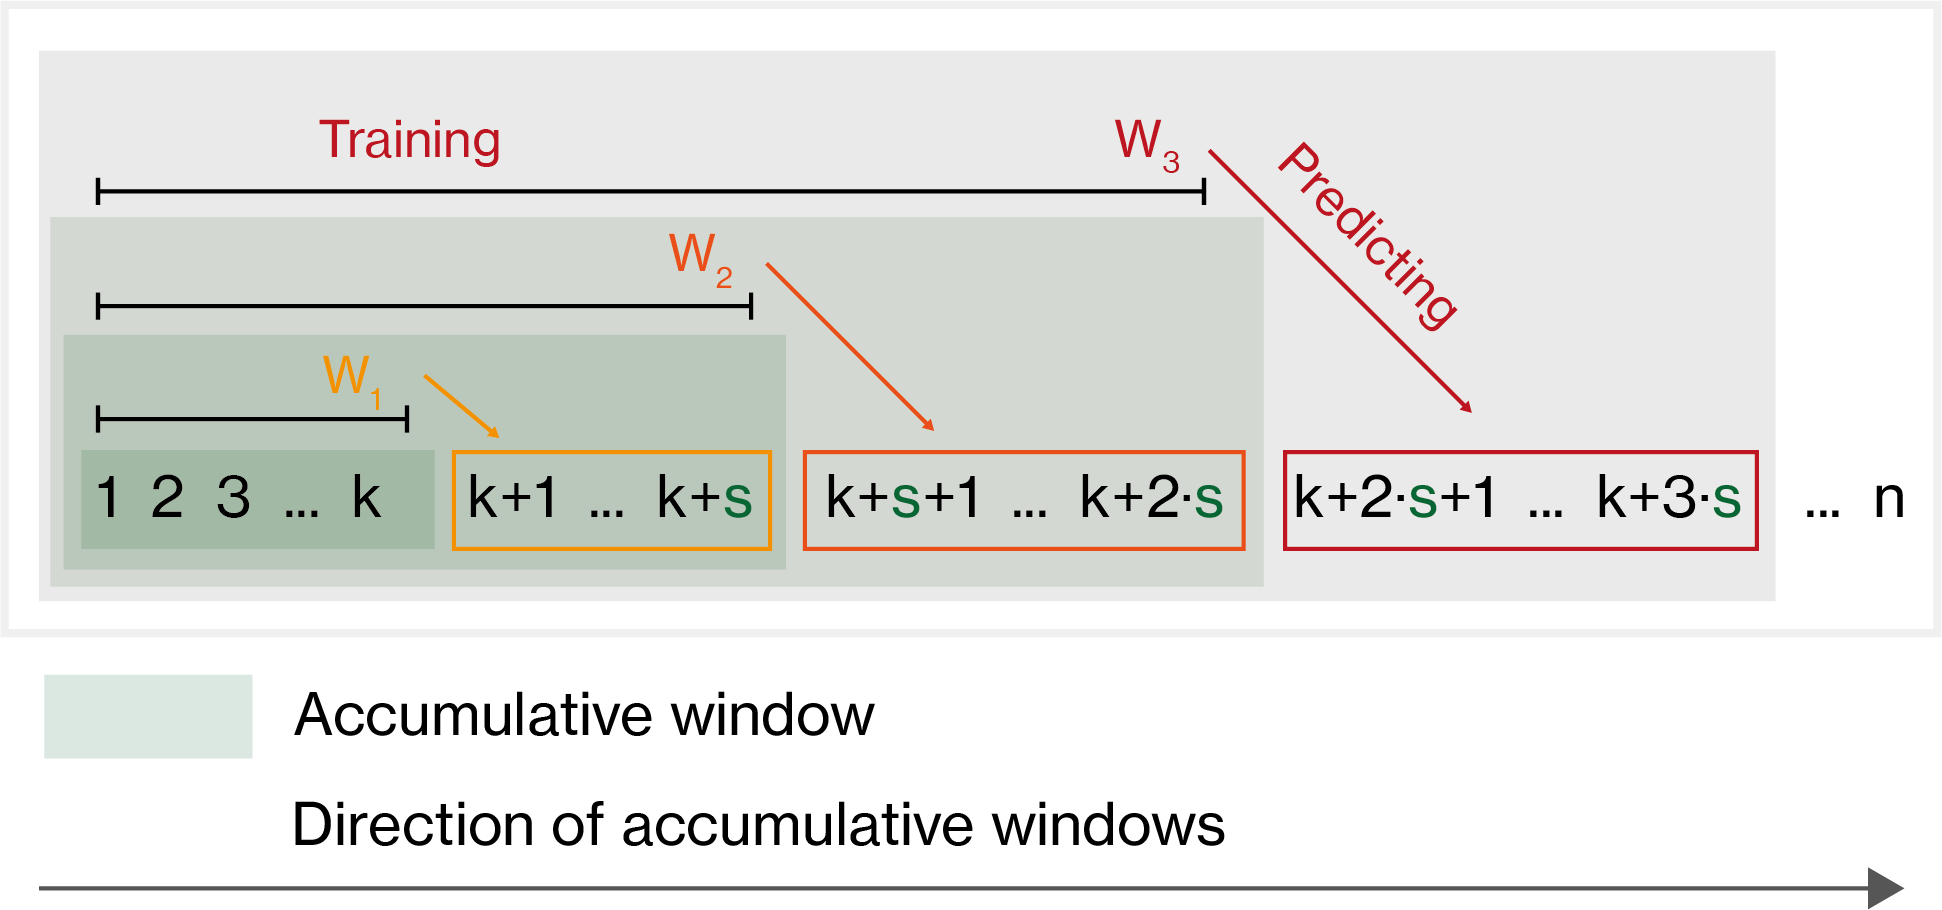
\includegraphics[width=0.55\textwidth]{figures/Accumulative retraining.png}
  \caption{\textit{Accumulative training diagram.} $W$ represents the windows for each training, $s$ is the prediction steps. In this study, the initial $W_1$ is 61080 steps (data of year 2017 and 2018) and $s$ is 96 steps (data of one day). }
  \label{fig:Accumulative}
\end{figure}

Linear regression is a statistical modeling technique used to establish a linear relationship between a dependent variable and one or more independent variables. It assumes a linear relationship between the variables and aims to find the best-fit line that minimizes the difference between the predicted values and the actual values. Linear regression is widely used for forecasting and prediction tasks because of its capability to achieve reliable predictive performance and cross-compatibility\cite{city_scale_pred}, especially when the relationship between the variables is believed to be linear. Compared with other complicated machine learning techniques, training a LR model is fast, even when dealing with large data sets. Thus, online forecasting is feasible, which is also known as accumulative training. The process of accumulative training is shown in Fig. \ref{fig:Accumulative}. This method gradually expands the size of training data without overflowing historical data. Increasing training data can reduce the prediction errors\cite{online_LR}. We denote MPC with forecasts generated by this method as \textbf{MPC-LR}. Furthermore, we execute an additional forecasting technique utilizing LR by incorporating covariates namely time characteristics and meteorological data. The designation for MPC utilizing this forecast is \textbf{MPC-LRCo}.

\subsubsection{Probabilistic forecasting with autoregressive recurrent networks (DeepAR)}
% Machine learning - Probabilistic forecasting with autoregressive recurrent networks

Probabilistic forecasting with autoregressive recurrent networks (DeepAR) is a method that combines autoregressive models and recurrent neural networks (RNNs) to make probabilistic predictions. In some cases, long short-term memory (LSTM) can be used to replace the RNN. AR models capture dependencies between past and current observations, while RNNs are designed to model sequential data. By combining these two techniques, probabilistic forecasting with AR networks can generate predictions along with a measure of uncertainty, providing a probabilistic distribution of future values. DeepAR is good at learning seasonal behaviors and dependencies on given covariates across time series. At the same time, little manual intervention in providing covariates is needed in order to capture complex behaviors\cite{DeepAR}. In this method, only future covariates (i.e. time features) are encoded due to the limitation of RNN model. MPC with this prediction is denoted as \textbf{MPC-DeepAR}.

\subsubsection{Temporal Fusion Transformer (TFT)}
% Machine learning - Temporal fusion transformer

The Temporal Fusion Transformer (TFT) is a forecasting model that combines elements of recurrent neural networks and transformers. It is designed to capture complex temporal patterns in time series data. TFT uses a hierarchical architecture that includes encoder-decoder layers, attention mechanisms, and gating mechanisms. It can handle multiple time series inputs and can model long-range dependencies effectively. TFT has been shown to deliver accurate and interpretable predictions for various forecasting tasks\cite{TFT}. Major constituents of TFT related to our forecasting task include gating mechanisms, variable selection networks and temporal processing. Gating mechanisms and variable selection networks help select relevant input variables at each time step. In the temporal processing mechanism, a sequence-to-sequence layer is employed for local processing of short-term dependencies, while long-term temporal relations are captured using a novel interpretable multi-head attention block.  MPC with this prediction is denoted as \textbf{MPC-TFT}.

\subsubsection{Extreme Gradient Boosting (XGBoost)}
% Machine learning - Extreme gradient boosting 

Extreme Gradient Boosting (XGBoost) is a popular machine learning algorithm known for its efficiency and predictive power. XGBoost is an ensemble method that combines multiple weak prediction models, typically decision trees, into a strong predictive model. It uses gradient boosting, which sequentially trains models by focusing on the errors made by previous models \cite{XGBoost}. XGBoost incorporates regularization techniques to prevent overfitting and provides high accuracy for various prediction tasks, including regression and classification. XGBoost is widely used for building-scale\cite{wang2020building} and city-scale\cite{wang2021predicting} load forecasting, and is also a frequent winner in Kaggle forecasting competitions\cite{Kaggle}. Its performance mainly attributes to these innovations: the tree-learning algorithm boosting sparse data process, a theoretically justified weighted quantile sketch procedure enabling approximate tree learning, and parallelisation together with distributed computing shrinking the training time. Benefited by the tree-learning algorithm, both meteorological and time feature covariates are utilized in XGBoost training. MPC with this prediction is denoted as \textbf{MPC-XGBoost}.

\subsubsection{Hyperparameter tuning}

For machine learning tasks, hyperparameter searching is a cumbersome and time consuming process. Due to model complexity and large size of training data, conventional grid-search approach is not applicable in this study. Thus we chose \textit{Optuna}, an efficient way of hyperparameter tuning adopting efficient searching and pruning algorithms\cite{optuna_2019}, as our hyperparameter tuning method. Corresponding configurations for DeepAR, TFT and XGBoost are listed in Table. \ref{tab:Optuna}.

\begin{table}\centering
\renewcommand\arraystretch{1} %行高为1.5倍
\setlength{\abovecaptionskip}{10pt}
\setlength{\belowcaptionskip}{-10pt}
\begin{tabular}{cccc}
   \toprule
   % & T & Models &  &  \\
   Model parameters & TFT & DeepAR & XGBoost   \\
   \midrule
   used covariates & $CO^T$ & $CO^T$ & $CO^T$, $CO^M$  \\ 
   epochs & [1, 100] & [1, 50] & [1, 250]   \\
   optimization trials & 100 & 100 & 30   \\
   learning rate & [$10^{-4}$, 1] & [$10^{-4}$, 1] & [$10^{-3}$, 1] \\
   batch size & 96 & [8, 672] & - \\
   dropout rate & [0.01, 1] & [0.01, 1] & - \\
   \midrule
   % input chunk length & 672 & 672 & - \\
   % output chunk length & 96 & 96 & - \\
   % gradient clip & 0.1 & 0.1 & - \\
   RNN layers & - & [1, 8] & - \\
   \midrule
   LSTM layers & [1, 8] & - & - \\
   hidden dimensions & [1, 8] & - & - \\
   attention heads & [1, 8] & - & - \\
   \midrule
   minimum child weight & - & - & [5, 10] \\
    maximum depth& -& -&[1, 5]\\
    gamma& -& -&[0.25, 1]\\
    subsample  & -& -&[0.01, 0.2]\\
    colsample bytree& -& -&[0.01, 0.2]\\
    regularization alpha& -& -&[$10^{-8}$, 1]\\
    regularization lambda& -& -&[$10^{-8}$, 1]\\
    \bottomrule
\end{tabular}
\caption{Hyperparameters for \emph{Optuna} searching}\centering
    \label{tab:Optuna}
\end{table}


\subsubsection{Adaptive moving average (AMA)}

In contrast with \emph{machine learning} approaches, \emph{heuristic} methods are simple and intuitive. We adopt a quite simple heuristic model for building load forecast. Specifically, the estimate for time step $t+k$ forecast at time $t$:
\begin{equation}
    \bldest_{t+k \mid t} = \alpha^k \pbld_{t-1} + (1 - \alpha^k) \bldavg_{\tset(t+k)} 
\end{equation}
where $\bldavg_{\mathcal{A}} = \frac{1}{\abs{\mathcal{A}}}\sum_{t\in \mathcal{A}} \pbld_t$ is the average of some selected historical data, and for our specific choice, $\tset(t)$ is the set of the most recent four steps whose day-of-week (DoW) and time-of-day (ToD) are the same as $t$. We pick $\alpha = 0.1$. 
Since it combines last observed data with exponentially decaying historical data as the prediction window moving forward, we call this implementation as adaptive moving average (AMA). MPC with this prediction is denoted as \textbf{MPC-AMA}.

% The overall prediction MAPE is 6.63\% in 2019.\footnote{Our model is adaptive since we include the last time step $\pbld_{t-1}$ as a reference, which is usually good estimate for very near future. MAPE for $k\le 4$ is 3.13\%, while MAPE for $48 < k\le 96$ is 6.90\% (1 hour contains 4 steps).} 

\subsubsection{Forecast accuracy}
    
The forecasting performances are primarily evaluated by using four (lump) metrics, as defined in Eqs. \eqref{eq:MAE}-\eqref{eq:CV-RMSE}, where $y_t$ and $\widehat{y_t}$ are actual and forecasting values. They are the mean absolute error (MAE), the root mean squared error (RMSE), the mean absolute percentage error (MAPE) and the coefficient of variation of the root mean squared error (CV-RMSE). MAE and RMSE are scale-dependent which can provide a straight-forward quantification to the readers, while MAPE and CV-RMSE are normalized metrics so it is more comparable across specific buildings. In addition, existing studies and guidelines provided some benchmarks for evaluating the model by using CV-RMSE. Specifically, resulting CV-RMSE below 30\% indicates the model is calibrated and sufficiently close to physical reality for engineering purposes when using hourly data\cite{CV-RMSE_standard}.  

\begin{figure}[!ht]
\centering
  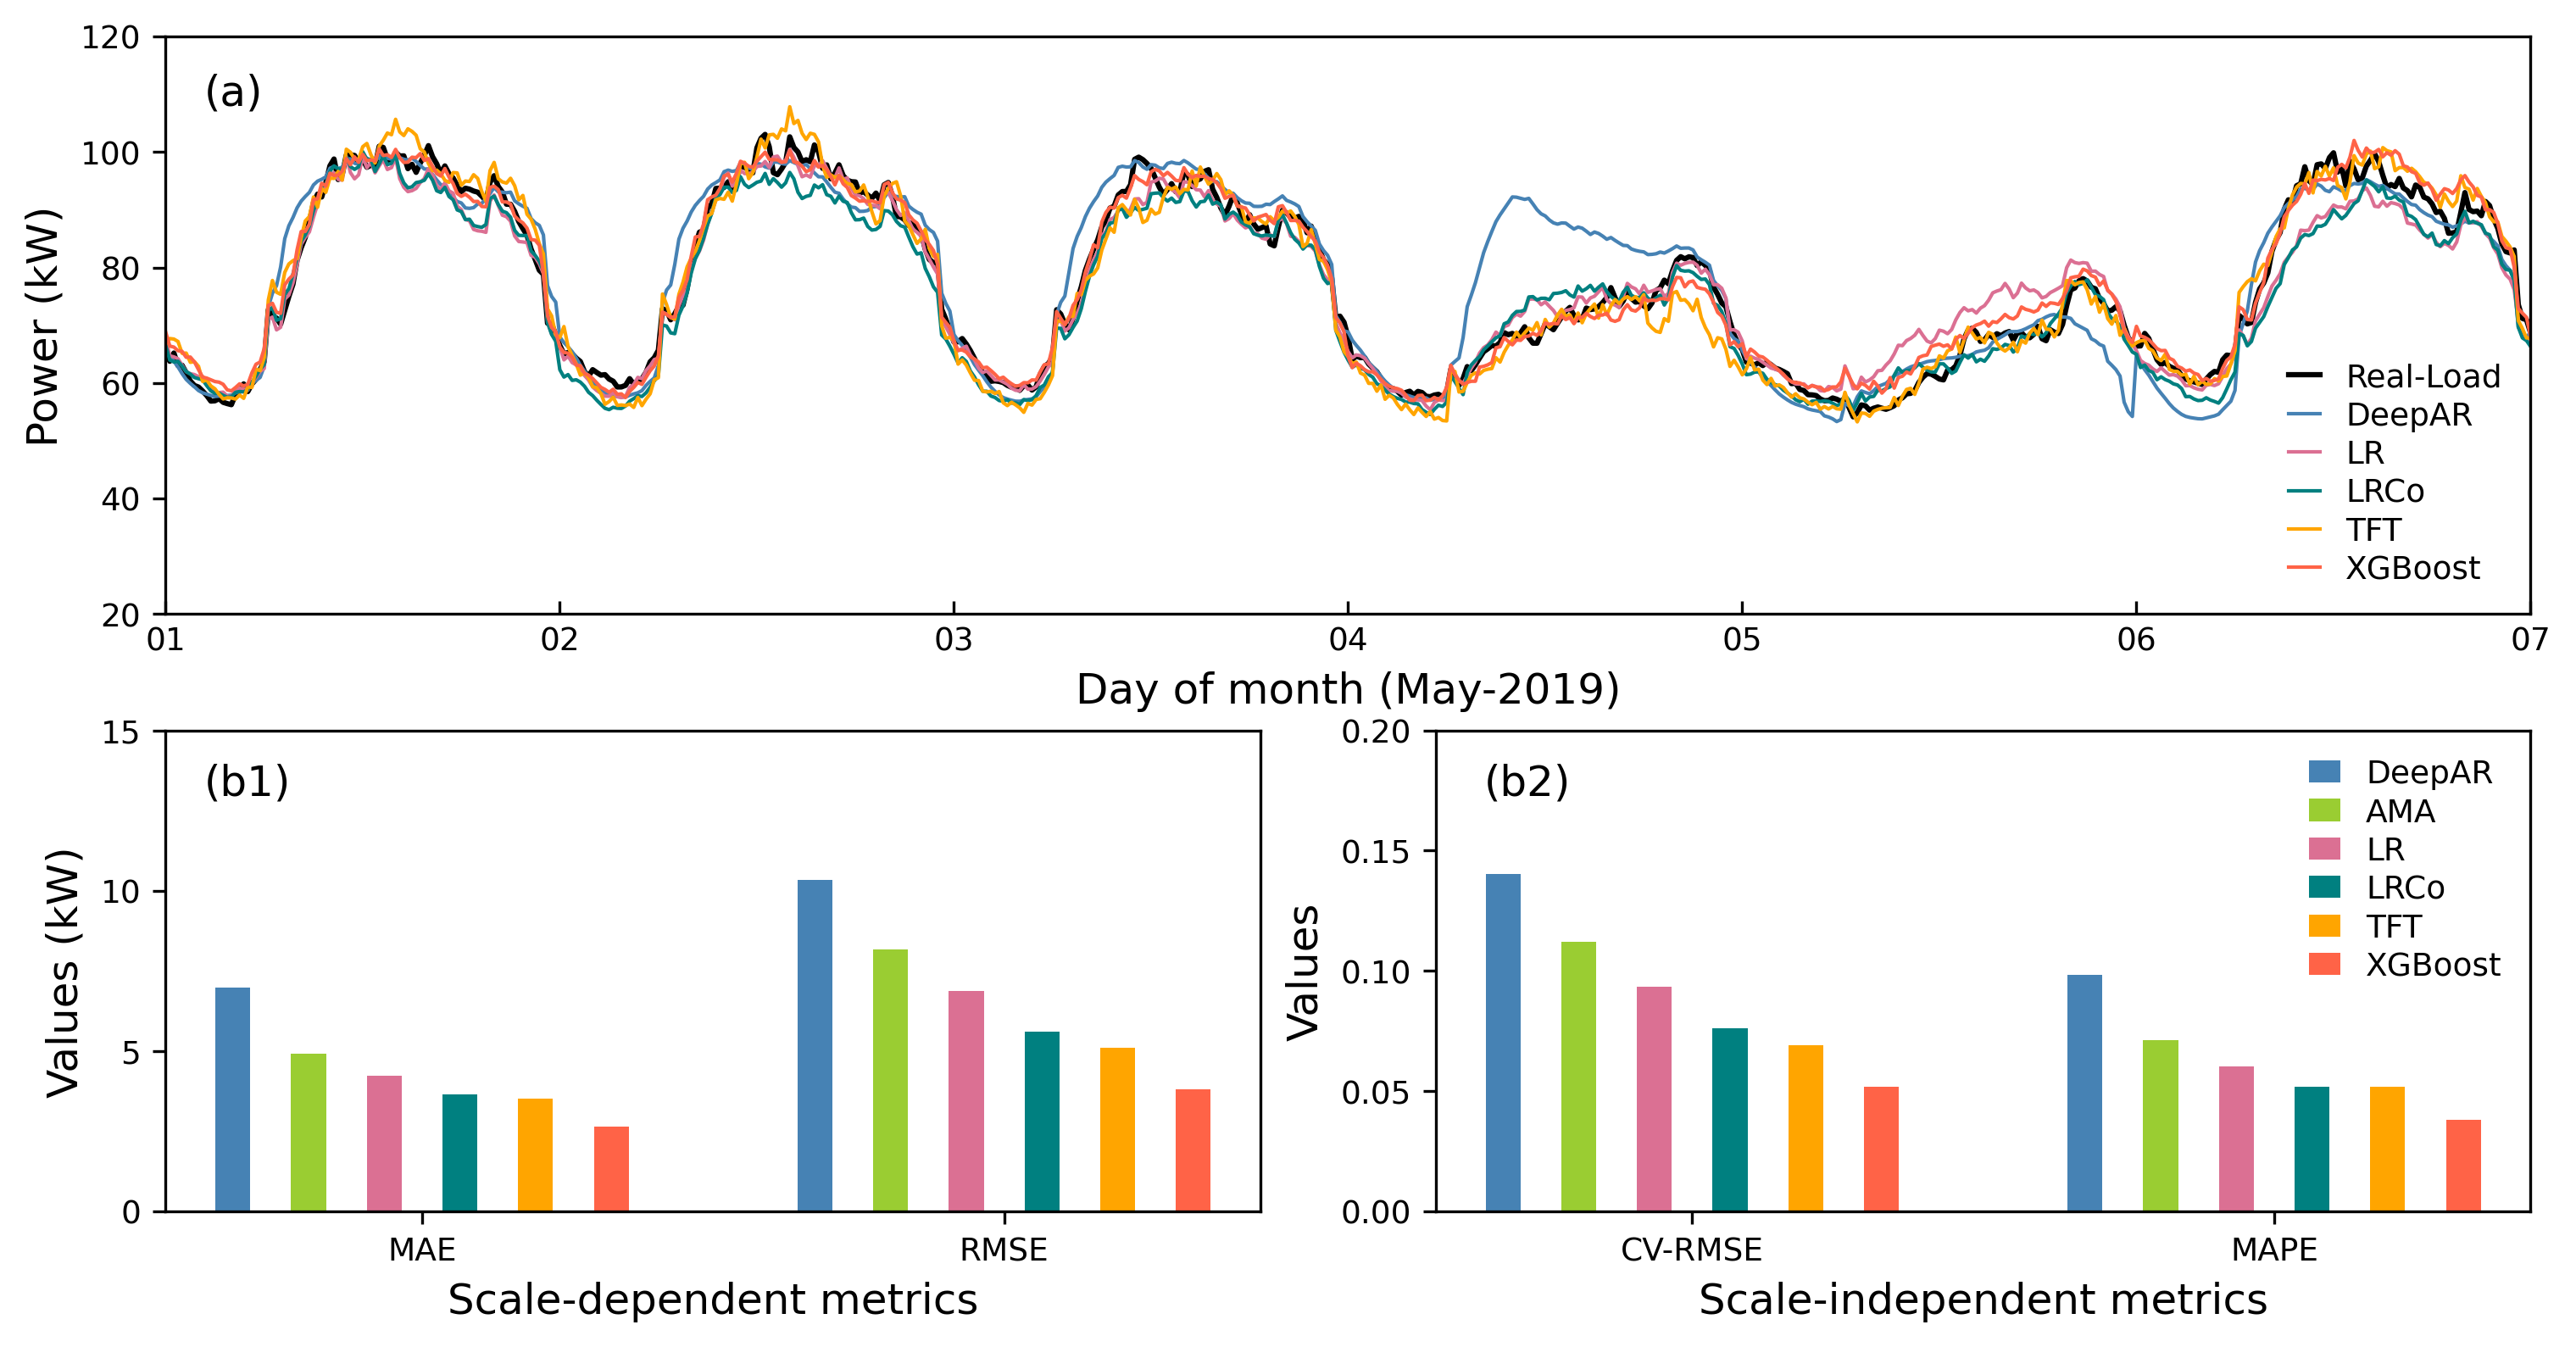
\includegraphics[width=0.85\textwidth]{figures/fig-1-load-prediction-and-metrics.png}
  \caption{\textit{Sample forecasts and error metrics} \textbf{(a)}. Real load values are represented by black line, and forecasts of different machine learning models are colored lines as tagged in legend. The AMA generates adaptive forecasts, which are not plotted in this figure. \textbf{(b1)-(b2)} Visualizing the scale-dependent and scale-independent metrics of different forecasts. }
  \label{fig:prediction}
\end{figure}

\begin{equation} \label{eq:MAE}
    MAE = \frac{1}{n} \sum_{t=1}^{n}\abs{y_{t}-\widehat{y_{t}}}
\end{equation}

\begin{equation}
    RMSE = \frac{1}{n} \sqrt {\sum_{t=1}^{n}(y_{t}-\widehat{y_{t}})^{2}}
\end{equation}

\begin{equation}
    MAPE = \frac{1}{n}\sum_{t=1}^{n} \abs{\frac{y_t-\widehat{y}_t}{y_t}}
\end{equation}
    
\begin{equation} \label{eq:CV-RMSE}
    CV-RMSE = \frac{\sqrt{\frac{\sum_{t=1}^{n}(y_{t}-\widehat{y_{t}})^{2}}{n}}} {\frac{\sum_{t=1}^{n} y_{t}}{n}}
\end{equation}

%\lunlong{Explanations for forecasting results will be added.}
  
% \lunlong{Maybe the explanation of OPEX, TOU should be placed here?}
%In this paper, we denote the set of real numbers by $\R$ and the set of integers by $\Z$. We use functions $\ind{\cdot}$, $[\cdot]^{+}$, $[\cdot]^{-}$, $\lfloor \cdot \rfloor$ in their conventional meanings, i.e., $\ind{x}=1$ if $x$ is true otherwise $\ind{x}=0$, $[x]^{+} \coloneqq \max\{0,x\}$, $[x]^{-} \coloneqq \min\{0,x\}$.\footnote{For consistency, we adopt the convention that using lowercase letters (e.g., $x$) for (decision) variables, uppercase letters (e.g., $X$) and Greek letters (e.g., $\alpha$) for parameters, and calligraphic uppercase letters (e.g., $\mathcal{X}$) for sets.}
Fig. \ref{fig:prediction}. provides sample forecasts of a week, and summarizes the resulting MAE, RMSE, CV-RMSE and MAPE. In general, all forecasting models outperform the threshold of 30\% in terms of CV-RMSE, showcasing a range from 5.17\% to 14.04\%. Compared to performances provided by other related research \cite{hourly_building_cooling_load_pred}, the resulting CV-RMSE is lower. This enhanced performance can be attributed to the nature of the building load data employed in this study, which represents the average demand of eight individual buildings. This aggregation serves to mitigate the inherent uncertainty in load patterns, resulting in more robust forecasting outcomes.
Among all accessed methods, XGBoost emerges as the frontrunner, exhibiting superior performance with a MAPE of 3.80\%. TFT has the resulting MAPE of 5.19\% inferior to XGBoost. Though the structure of LR is rather simple, it exerts good performance of 6.01\% (MAPE), as a result of constantly retraining. By encoding covariates, the MAPE of LRCo is enhanced to 5.18\%. Of particular note is the heuristic method AMA, which defies expectations with its robust performance, despite its simplicity. Leveraging observations from the preceding time step, AMA attains a MAPE of 7.13\%, surpassing the performance of the more intricate DeepAR model, which registers a MAPE of 9.83\%.

%============================================================================================================
\subsection{Simulation configurations}
\label{section:configurations}
Based on streamed PV and building load data and corresponding forecasts in the year of 2019, the simulations are performed under two scenarios ($\wodc$ and $\wdc$) to examine the impact of pricing schemes. Under $\wodc$ (without demand charge), the utility bills consists of only TOU (time of use) costs, where the demand charge rate $\dc$ was set as $0$ \$/kW. Under $\wdc$ (with demand charge), the demand charge rate $\dc$ was set as $18$ \$/kW in a billing cycle of one month, representing a typical scenario in California. Apart from the demand charge rate $\dc$, other configurations for both scenarios are set as follows: 
 
In order to make our analysis more generalizable, we intentionally rescaled the annual PV generation and the battery capacity, then they are proportional to the annual building load. The factors, namely $\rpv$ and $\rbat$ were set as 50\% and 6h in this study. Battery (dis)charging efficiencies were set as $0.98$. 
We used the day-ahead price (DA) of San Diego Gas \& Electric (SDGE) as the grid TOU $\tou^+$\footnote{Considering the price difference between wholesale markets and business plans, we rescaled TOU so that its average was $0.17$ \$/kWh. We assume DA is known.}. Selling prices $\tou^-$ were set as fixed proportion to buying prices $\tou^+$, and the factor was $0.6$ in our base case.
%============================================================================================================